\chapter{构建阀瓣三维模型}

{\bfseries 学习目标}
\begin{itemize}
\item 学习利用chamfer命令编辑图形
\item 学习利用copy命令编辑图形
\item 学习利用Move命令绘编辑图形
\item 学习利用cone命令建立圆锥体
\end{itemize}

{\bfseries 任务要求}
\begin{itemize}
\item 根据图\ref{fig:tiaoyafafaban}所示的杯零件图,用实体建模法建立调压阀阀瓣零件的三维模型
\end{itemize}

\noindent
\begin{figure}[htbp]
\centering
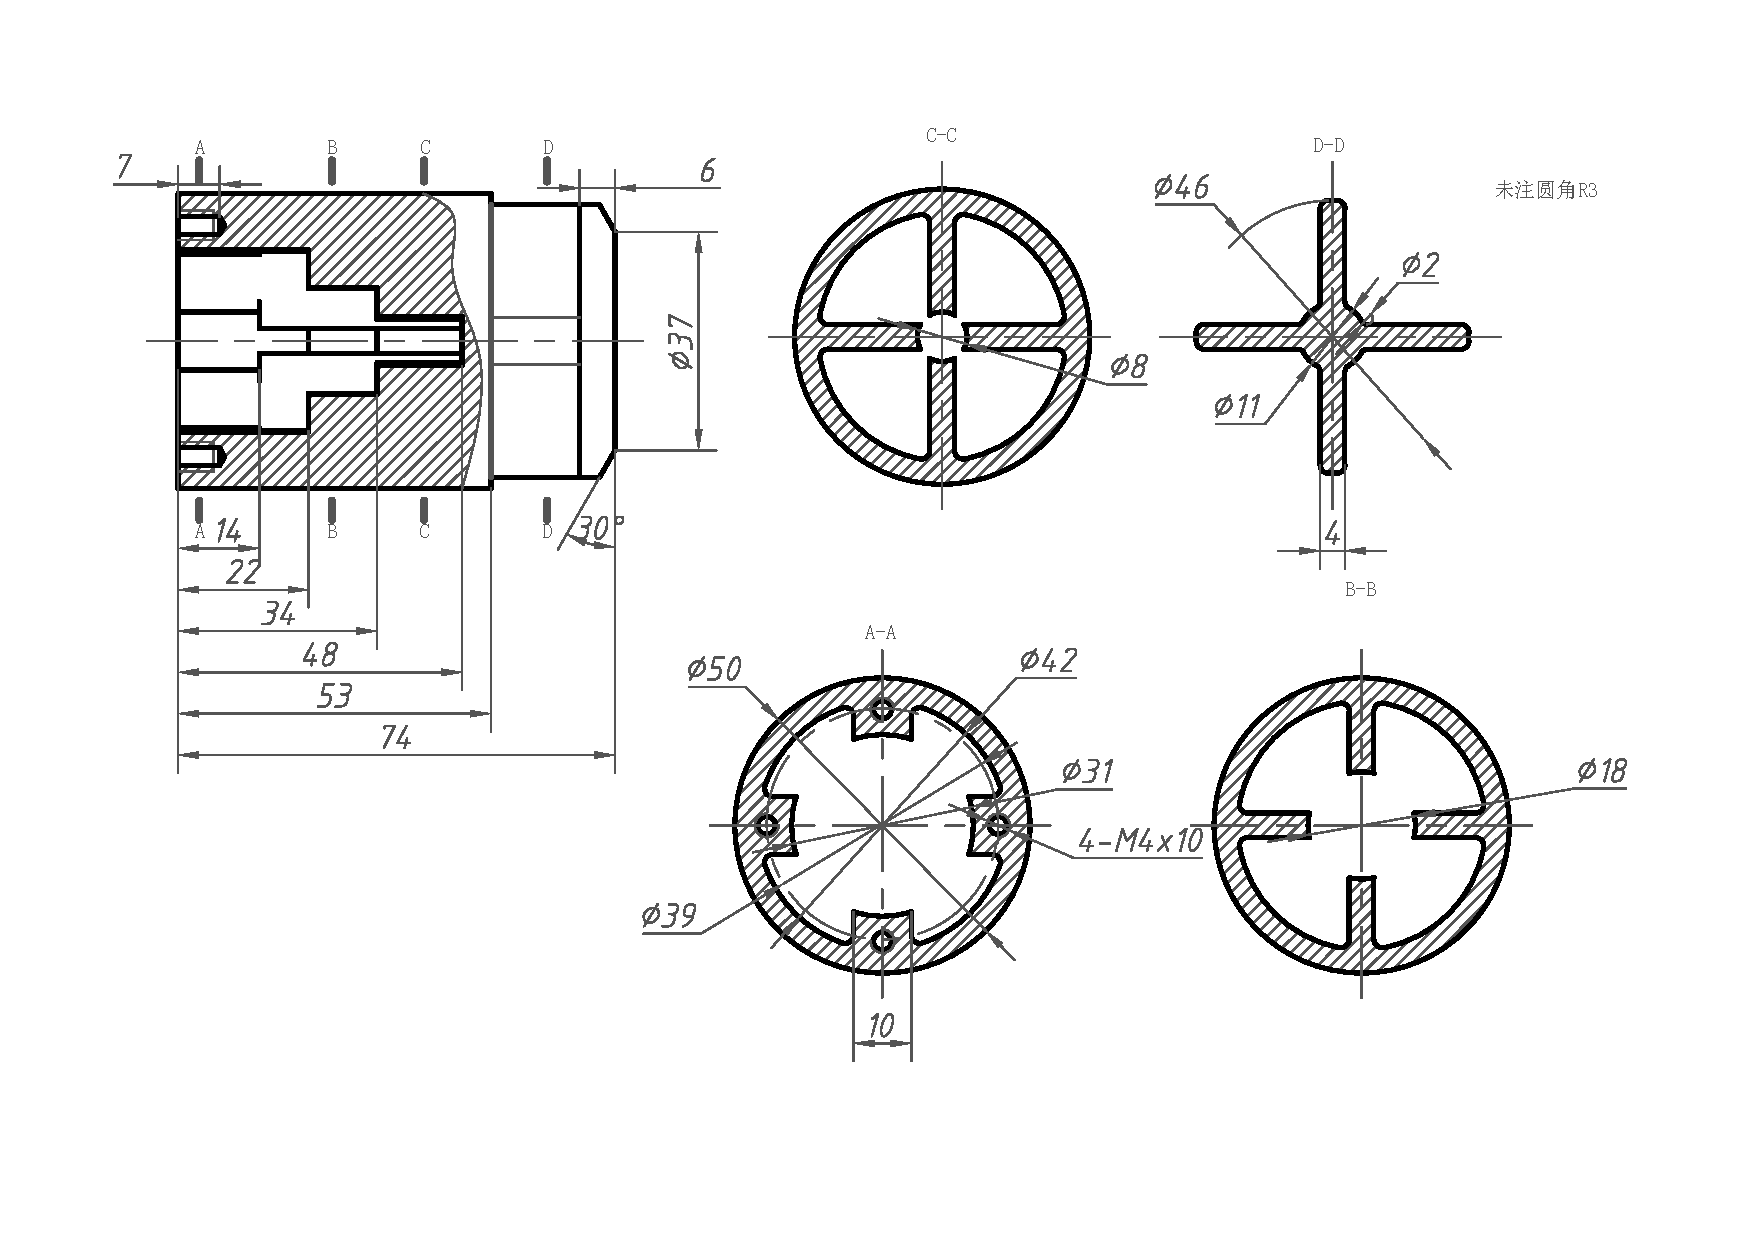
\includegraphics[scale=0.45]{tiaoyafafaban.pdf}
\caption{阀瓣零件图}\label{fig:tiaoyafafaban}
\end{figure}
\endinput